\documentclass[portrait]{tikzposter}

%TODO: nullfont ?  Dès le début de l'usage de tikzposter !
%TODO: various font subst to investigate

\usepackage{hyperref}
\usepackage{pgfplots}
\usepackage{tkz-euclide}% for geometry
\usepackage{tikz-qtree}
\usepackage{lipsum}% for dummy text
\usepackage{multicol}% for multiple columns
\setlength{\columnsep}{4cm}
\setlength{\columnseprule}{1mm}
\usepackage{amsmath}

\newcommand{\myvspace}{\vspace{0.5cm}}
\newcommand{\rank}{\text{rank}}
\newcommand{\defblock}[2]{
 \colorlet{innerblocktitlebgcolor}{colorFour}
 \innerblock{#1}{#2}
 \colorlet{innerblocktitlebgcolor}{colorThree}
}

\definecolor{colorFour}{HTML}{008000} %green
\definelayouttheme{MyBoard}{
    \usecolorstyle[colorPalette=BlueGrayOrange]{Spain}
    \usebackgroundstyle{Default}
    \usetitlestyle{Default}
    \useblockstyle{Basic}
    \useinnerblockstyle{Envelope}
    \usenotestyle{Sticky}
}

\usetheme{MyBoard}
\colorlet{backgroundcolor}{white}

\pgfplotsset{compat=1.18}

\usetikzlibrary{lindenmayersystems,shadings}% gives us fractals
%\pgfdeclarelindenmayersystem{Koch curve}{
%  \rule{F -> F-F++F-F}}
%\pgfdeclarelindenmayersystem{Sierpinski triangle}{
%  \rule{F -> G-F-G}
%  \rule{G -> F+G+F}}
%\pgfdeclarelindenmayersystem{Fractal plant}{
%  \rule{X -> F-[[X]+X]+F[+FX]-X}
%  \rule{F -> FF}}
%\pgfdeclarelindenmayersystem{Hilbert curve}{
%  \rule{L -> +RF-LFL-FR+}
%  \rule{R -> -LF+RFR+FL-}}

\title{\huge Some Curious Recursive Functions : Hostadter's G and After}
\author{Pierre Letouzey (équipe ACS, ...)}
\institute{IRIF, Université Paris Cité / Picube, INRIA / CNRS}

%% Insert logos to the left and right of tkizposter title
%% Source: StackOverflow

\makeatletter
\newcommand\insertlogoi[2][]{\def\@insertlogoi{\includegraphics[#1]{#2}}}
\newcommand\insertlogoii[2][]{\def\@insertlogoii{\includegraphics[#1]{#2}}}
\newlength\LogoSep
\setlength\LogoSep{0pt}

\renewcommand\maketitle[1][]{  % #1 keys
    \normalsize
    \setkeys{title}{#1}
    % Title dummy to get title height
    \node[transparent,inner sep=\TP@titleinnersep, line width=\TP@titlelinewidth, anchor=north, minimum width=\TP@visibletextwidth-2\TP@titleinnersep]
        (TP@title) at ($(0, 0.5\textheight-\TP@titletotopverticalspace)$) {\parbox{\TP@titlewidth-2\TP@titleinnersep}{\TP@maketitle}};
    \draw let \p1 = ($(TP@title.north)-(TP@title.south)$) in node {
        \setlength{\TP@titleheight}{\y1}
        \setlength{\titleheight}{\y1}
        \global\TP@titleheight=\TP@titleheight
        \global\titleheight=\titleheight
    };

    % Compute title position
    \setlength{\titleposleft}{-0.5\titlewidth}
    \setlength{\titleposright}{\titleposleft+\titlewidth}
    \setlength{\titlepostop}{0.5\textheight-\TP@titletotopverticalspace}
    \setlength{\titleposbottom}{\titlepostop-\titleheight}

    % Title style (background)
    \TP@titlestyle

    % Title node
    \node[inner sep=\TP@titleinnersep, line width=\TP@titlelinewidth, anchor=north, minimum width=\TP@visibletextwidth-2\TP@titleinnersep]
        at (0,0.5\textheight-\TP@titletotopverticalspace)
        (title)
        {\parbox{\TP@titlewidth-2\TP@titleinnersep}{\TP@maketitle}};

    \node[inner sep=0pt,anchor=west]
      at ([xshift=-\LogoSep]title.west)
      {\@insertlogoi};

    \node[inner sep=0pt,anchor=east]
      at ([xshift=\LogoSep]title.east)
      {\@insertlogoii};

    % Settings for blocks
    \normalsize
    \setlength{\TP@blocktop}{\titleposbottom-\TP@titletoblockverticalspace}
}
\makeatother


\insertlogoi[width=9cm]{logo-irif.pdf}
\insertlogoii[width=9cm]{logo-3tutelles.pdf}

\begin{document}
\maketitle

\begin{columns}


  \column{.33}%GAUCHE
\block{Nested Recursions}{

From the book "Gödel,Escher,Bach" \cite{GEB} :
%TODO Proper ref

\medskip
\defblock{Definition: Hofstadter's G function}{
\begin{equation*}
\begin{cases}
G(0) = 0 \\
G(n) = n - G(G(n-1)) \hspace{4cm} \text{for all}\ n>0
\end{cases}
\end{equation*}
}

\medskip

More generally, with $k+1$ nested recursive calls:

\medskip

\defblock{Definition: the $F_k$ functions}{
\begin{equation*}
\begin{cases}
F_k(0) = 0 \\
F_k(n) = n - F_k^{(k+1)}(n-1) \hspace{4cm} \text{for all}\ n>0
\end{cases}
\end{equation*}
}

\myvspace

\pgfplotsset{width=\linewidth}
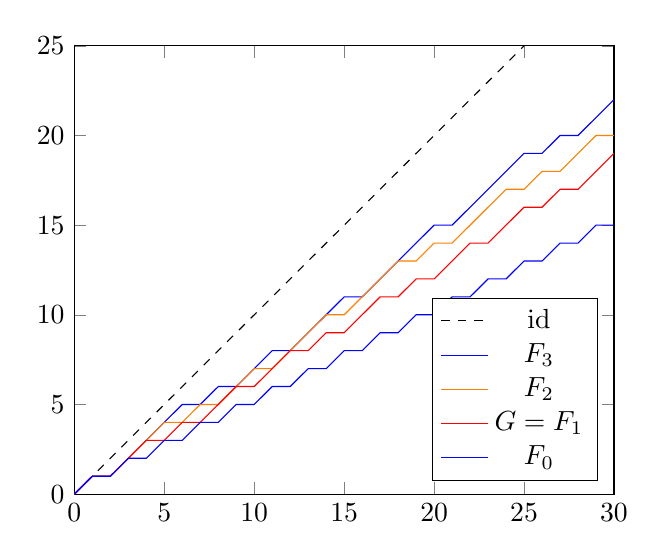
\begin{tikzpicture}[scale=1]
  \begin{axis}[
    xmin=0,xmax=30,ymin=0,ymax=25,samples=31,
    xtick = {0,5,...,30},
    ytick = {0,5,...,30},
    %xlabel=$n$,
    legend pos=south east
  ]

 \addplot+[mark=.,color=black,style=dashed,domain=0:30] {x};
 \addlegendentry{id}
    \addplot [mark=.,color=blue] coordinates {
(0, 0) (1, 1) (2, 1) (3, 2) (4, 3) (5, 4) (6, 5) (7, 5) (8, 6)
 (9, 6) (10, 7) (11, 8) (12, 8) (13, 9) (14, 10) (15, 11) (16, 11)
 (17, 12) (18, 13) (19, 14) (20, 15) (21, 15) (22, 16) (23, 17)
 (24, 18) (25, 19) (26, 19) (27, 20) (28, 20) (29, 21) (30, 22)};
 \addlegendentry{$F_3$}
    \addplot [mark=.,color=orange] coordinates {
(0, 0) (1, 1) (2, 1) (3, 2) (4, 3) (5, 4) (6, 4) (7, 5) (8, 5)
 (9, 6) (10, 7) (11, 7) (12, 8) (13, 9) (14, 10) (15, 10) (16, 11)
 (17, 12) (18, 13) (19, 13) (20, 14) (21, 14) (22, 15) (23, 16)
 (24, 17) (25, 17) (26, 18) (27, 18) (28, 19) (29, 20) (30, 20) };
 \addlegendentry{$F_2$}
 \addplot+[mark=.,domain=0:30,color=red]
 {floor((x+1) * 0.618033988749894903)};
 \addlegendentry{$G=F_1$}
 \addplot+[mark=.,domain=0:30] {ceil(x/2)};
 \addlegendentry{$F_0$}
 \end{axis}
\end{tikzpicture}

\myvspace

\innerblock{ Theorem (with Shuo Li, nov. 2023!): }
{$\forall k,\forall n, F_k(n) \le F_{k+1}(n)$}
}%block
%\note[targetoffsetx = 3cm, targetoffsety = -20cm,
%       angle = -30, connection, width=12cm]{\Large Nov~2023:~Proved! }


\block{Fibonacci-like Sequences}{

For any $k\ge 0$:

\myvspace

\defblock{Definition: the $A_k$ sequences}{
\begin{equation*}
\begin{cases}
A^k_n = n+1 \hfill \text{when}\ n\le k \\
A^k_{n+1} = A^k_{n} + A^k_{n-k} \hspace{5cm} \text{when}\ n+1 > k
\end{cases}
\end{equation*}
}

\myvspace

\begin{itemize}
\item $A^0$ : 1  2  4  8  16  32  64  128  256 $\ldots$
\item $A^1$ : 1  2  3  5  8  13  21  34  55  89 $\ldots$ (Fibonacci)
\item $A^2$ : 1  2  3  4  6  9  13  19  28  41 $\ldots$ (Narayana's Cows)
\item $A^3$ : 1  2  3  4  5  7  10  14  19  26 $\ldots$
\end{itemize}

\myvspace

\innerblock{Theorem: $F_k$ shifts down $A^k$}
{$\forall k, \forall n, F_k(A^k_n) = A^k_{n-1}$}

}%block

\block{Numerical Systems}{

\newcommand{\Arest}{\ensuremath{\Sigma A^k_i}}

\innerblock{Theorem (Zeckendorf):}{
Let $k\ge 0$. All $n\ge 0$ has a unique canonical decomposition
  $\Arest$ (i.e. with indices $i$ apart by at least $k+1$).
}

\myvspace

\innerblock{Theorem: $F_k$ on decompositions}{
The function $F_k$ shifts down the indices of canonical
decompositions: $F_k(\Arest) = \Sigma A^k_{i-1}$ (with here $0-1 = 0$).
}

\myvspace

For instance for $k=2$ and $n=18$ :
\begin{itemize}
\item $18 = A^2_0 + A^2_3 + A^2_6 = 1 + 4 + 13$
\item $F_3(18) = A^2_0 + A^2_2 + A^2_5 = 1 + 3 + 9 = 13$
\item $1+3+9$ no more canonical, possible renormalization
\end{itemize}

\myvspace

\defblock{Definition: rank}{
$\rank_k(n)$ : lowest index in the $k$-decomposition of $n$
}

\myvspace

\innerblock{Theorem: $F_k$ flat spots}{
$F_k(n)=F_k(n+1)$ iff $\rank_k(n) = 0$ (i.e. $n = 1 + \Arest$)
}

}%block


\column{.33}%CENTRE

\block{G as a Rational Tree}{

Let's repeat this branch pattern:

\myvspace

\begin{tabular}{lclclclc}
T & = & \hspace{-1cm}
\begin{tikzpicture}[grow'=up, level distance=2cm]
\Tree
     [.$\circ$ T
        [.$\circ$ [.T ]]]
\end{tikzpicture}
& = & \hspace{-1cm}
\begin{tikzpicture}[grow'=up, level distance=2cm]
\Tree
     [.$\circ$
       [.$\circ$ T
          [.$\circ$ [.T ]]]
       [.$\circ$ [.$\circ$ T
          [.$\circ$ [.T ]]]]]
\end{tikzpicture}
& = & \hspace{-1cm}
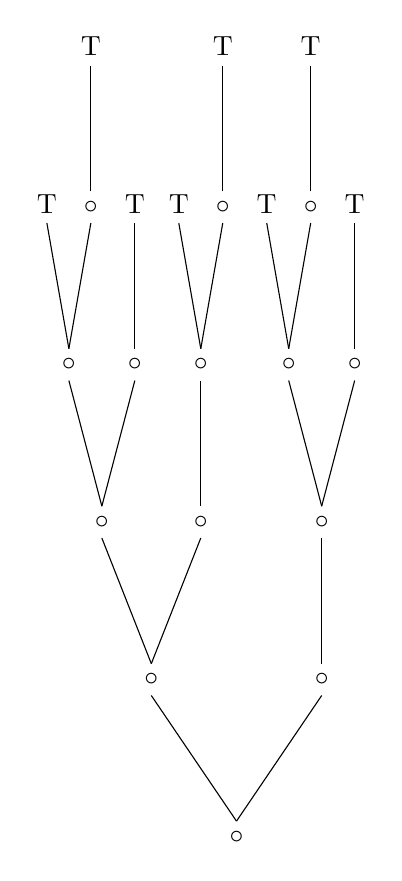
\begin{tikzpicture}[grow'=up, level distance=2cm]
\Tree
     [.$\circ$
       [.$\circ$ [.$\circ$ [.$\circ$ T
                                     [.$\circ$ T ] ]
               [.$\circ$ [.T ]]]
           [.$\circ$ [.$\circ$ T
                                           [.$\circ$ T ]]]]
       [.$\circ$ [.$\circ$ [.$\circ$ T
                                     [.$\circ$ T ]]
               [.$\circ$ T ]]]]
\end{tikzpicture}
& \hspace{-3cm} = $\ldots$

\end{tabular}

\myvspace

Now, with an ad-hoc trunk and node numbered via BFS:

\myvspace

\begin{tikzpicture}[grow'=up,level distance=2.5cm]

\bigskip
\bigskip

\Tree
 [.1 [.2 [.3
       [.4 [.6 [.9 [.14 22 23 ] [.15 24 ] ]
               [.10 [.16 25 26 ]]]
           [.7 [.11 [.17 27 28 ] [.18 29 ]]]]
       [.5 [.8 [.12 [.19 30 31 ] [.20 32 ]]
               [.13 [.21 33 34 ]]]]]]]
\end{tikzpicture}

\myvspace

\innerblock{Theorem:}{For any node $n>1$, its ancestor is $G(n)$. }

\myvspace

\innerblock{Exercise:}{ Which trees correspond to functions $F_k$ ? }

}%block

\block{Linear Equivalents}{

Let $\tau_k$ be the positive root of $X^{k+1}+X-1$. It is hence
algebraic, and irrational except for $k=0$.

\myvspace

\innerblock{Theorem:}{
For all $k\ge$, when $n\to\infty$ we have $F_k(n) = \tau_k.n + o(n)$
}

\myvspace
More precisely:
\myvspace

\coloredbox{
\begin{itemize}
\item $F_0(n) = \lfloor (n+1)/2 \rfloor = \lceil n/2 \rceil$
\end{itemize}}
And $A^0_n = 2^n$ and we retrieve the base-2 decomposition !

\myvspace

\coloredbox{
\begin{itemize}
\item $G(n) = F_1(n) = \lfloor \tau_1.(n+1) \rfloor$
\end{itemize}}
Here $\tau_1=1/\phi=\phi-1 \approx 0.618...$

\myvspace

\coloredbox{
\begin{itemize}
\item $F_2(n) - \lfloor \tau_2.n \rfloor \in \{0,1\}$
\end{itemize}}
Here $\tau_2 \approx 0.6823...$, inverse of Pisot number $P_3$. \\
Let $\delta(n) = F_2(n) - \tau_2.n$.
Then plotting $(\delta(i),\delta(F_2(i)))$
 leads to this Rauzy fractal\cite{Rauzy,Fogg}!

\includegraphics[width=\linewidth]{fractal.png}

\myvspace

\coloredbox{
\begin{itemize}
\item $F_3(n) - \lfloor \tau_3.n \rfloor \in \{-1,0,1,2\}$
\end{itemize}}
Here $\tau_3 \approx 0.7244...$, inverse of Pisot number $Q_3$.

\myvspace

\coloredbox{
\begin{itemize}
\item After $k\ge 4$, $F_k(n)-\tau_k.n = o(n)$ but not bounded.
\end{itemize}}
Note: $\tau_4$ is the inverse of the Plastic number (smallest Pisot),
then $\tau_k$ for $k\ge 5$ is above any Pisot inverse.


}%block

\column{.33}%DROITE

\block{Morphic Words}{

We take $\mathcal{A}=\{0..k\}$ as alphabet.

\myvspace

\defblock{Definition: the substitutions $\sigma_k$}{
\begin{equation*}
\begin{cases}
\mathcal{A} \to \mathcal{A}^* \\
\sigma_k(n) = n+1 \hspace{9cm} \text{for}\ n<k \\
\sigma_k(k) = k.0
\end{cases}
\end{equation*}
}

\myvspace

\defblock{Definition: the morphic words $m_k$}{

The substitution $\sigma_k$ is prolongeable at k. It hence admits
an infinite word $m_k$ (called \emph{morphic}) as fixed point:

$$m_k = \lim_{n\to\infty} \sigma_k^n(k) = \sigma_k(m_k) $$
}

\myvspace
For example:
\begin{itemize}
\item $m_1$ is the Fibonacci word (with opposite letters)
\item And $m_2 = 20122020120122012202...$
\end{itemize}

\myvspace

\innerblock{Theorem: alternative description of $m_k$}{
$m_k$ is also the limit of its finite prefixes $M^k_n$ defined as:
\begin{equation*}
\begin{cases}
M^k_n = k.0...(n-1) \hfill \text{for}\ n\le k \\
M^k_{n+1} = M^k_{n}.M^k_{n-k} \hspace{7cm} \text{for}\ n+1 > k
\end{cases}
\end{equation*}

Also note that $|M_{k,n}| = A^k_n$
}

\myvspace

\innerblock{Theorem: linear complexity}{
The subword complexity of $m_k$ (i.e. its number of distinct factors of
size $p$) is $p \mapsto k.p+1$.
}
In particular, $m_1$ is Sturmian (as expected).

\myvspace

\innerblock{Theorem: relating $m_k$ and $\rank_k$ and $F_k$}{
\begin{itemize}
\item At position $n>1$, $m_k[n] = min(k,\rank_k(n))$.
\item In particular this letter is 0 iff $F_k$ is flat there.
\item Hence the number of 0 in the $n$ first letters of $m_k$ is
  $n-F_k(n)$.
\item For any $p\le k$, counting the letters $\ge p$ gives
  $F_k^{(p)}$.
\item All letters in $m_k$ have (infinite) frequencies, for instance
  the frequency of 0 is $1-\tau_k$ (see Saari\cite{Saari}).
\end{itemize}
}

}%block

\block{Coq formalization}{
\begin{itemize}
\item Already $90\%$ of this poster certified in Coq:\\
\url{https://github.com/letouzey/hofstadter_g}

\item Nearly 20\,000 lines of Coq formalization

\item Several proved facts were just conjectures on OEIS.

\item At first, delicate (non-structural) function definitions over
  {\tt nat}, and many tedious recursions (multiple cases).

\item More recently, use of real and complex numbers, polynoms, matrix
  (e.g. Vandermonde and its determinant), some interval arithmetic for real
  approximation, etc.

\item Use the {\tt QuantumLib} library for its linear algebra part!

\end{itemize}
}%block

\block{Thanks!}{

A huge thanks to {\bf Paul-André Melliès}, one of the last
universalists, and to combinatorics experts {\bf Wolfgang Steiner},
and {\bf Yining Hu} and {\bf Shuo Li} !

}%block

\block{References}{
\normalsize
\vspace{-2.8cm}
\renewcommand{\refname}{}
\begin{thebibliography}{1}
\bibitem{GEB}
 Hofstadter, Douglas R.,
 {\it Gödel, Escher, Bach: An Eternal Golden Braid},
 1979, Basic Books, Inc, NY.

\bibitem{Fogg}
Pytheas Fogg, N.,
{\it Substitutions in Dynamics, Arithmetics and Combinatorics},
2002, LNCS 1794.

\bibitem{Saari}
Saari, K., {\it On the Frequency of Letters in Morphic
Sequences}, CSR 2006, LNCS 3967.

\bibitem{Rauzy}
Rauzy, G., {\it Nombres algébriques et substitutions}. Bulletin de la
SMF, Vol 110 (1982).
\end{thebibliography}
\vspace{-0.5cm}
}%block


\end{columns}

\end{document}
